% Chapter Template

\chapter{Arbitrage Theory In Continuous Time Finance} % Main chapter title

\label{Chapter2} % Change X to a consecutive number; for referencing this chapter elsewhere, use \ref{ChapterX}

Arbitrage theory in continuous time finance is a field with a lot of technical details from probability theory, where we follow the style in \parencite{Hull} and \parencite{finKont} to focus on intuition without going into the whelm of technicalities and proofs. The focus on this chapter will to provide the basic tools and intuition for the arbitrage theory and lay the foundations for the computational finance methods. The key question is how to price derivative fair and hedge the risk imposed by the derivative. The thesis will mainly deal with the former, where the concepts of arbitrage and compleness will be important.\\

We start with introducing the financial markets and key concepts for building arbitrage free and complete market models (see section \ref{FinMarket}). Then we actually build a framework for finding "fair" prices, i.e. finding a complete model with absense of arbitrage (see section \ref{MultiDimModel}). Lastly we go into specific cases where either a closed-form solution exist or numerical methods is needed(section \ref{classicBS} and \ref{AmericanOptions}).

%----------------------------------------------------------------------------------------
%	SECTION 1
%----------------------------------------------------------------------------------------

\section{Financial Markets}\label{FinMarket}
In the financial markets there is a lot of players and different types of investments. The classical investments are bonds and stocks, where the big players in the markets are commercial banks, investment banks, insurance companies and pension funds. Besides the classical investments types derivatives gives additional options for investments. A derivative are a financial instrument depending on an underlying asset, where the dependency is specified in the contract. The options in this thesis will all be stock options, but the techniques developed can easily be extended to other types of derivatives. To find prices of derivatives in modelling we restrict our financial market to d risky assets $\bm{S}(t)$ and a bank account $S_0(t)$ as numeraire. The probability space $(\Omega, \mathcal{F}, P)$ with a filtration $\mathbb{F}=(\mathcal{F}_t)_{t\geq 0}$ is the fundamental for modelling stochastic processes describing asset prices and trading strategies, where in the thesis the probability space $(\Omega, \mathcal{F}, \mathbb{F}, P)$ will be implicit assumed. Intuitively the filtration $\mathcal{F}_t$ is the information observable to time t, where the filtration $\mathbb{F}^{W}$ is often used in the thesis and it is be generated by the wiener processes $(W_t)_{0\leq t \leq T}$. The bank account is assumed to be a strictly positive adapted process $S_0=(S_0 (t))_{t \geq 0}$ and $S_0(0)=1$, where the d risky assets are modelled by a $\mathbb{R}^d$ adapted stochastic proces $\bm{S}=(\bm{S}(t))_{t\geq 0}$. The risky assets are in this thesis stocks by financial reasons the stocks are assumed positive $S_i(t)\geq 0$ P-a.s for all i and t. By using the bank account as numeraire i.e. dividing dividing the traded asset by the bank account ($\frac{\bm{S}(t)}{S_0 (t)}$), this amounts to working with \textit{zero interest}. We assume that the our financial market is frictionless, which contains a lot of assumptions.
\theoremstyle{assumption}
\begin{assumption}{}\label{EfficientMarket}
We assume following institutional facts:
\begin{enumerate}
\item[•] Short positions and fractional holding are allowed 
\item[•] There are no bid-ask spread, i.e. selling price is equal to buying price
\item[•] There are no transactions costs of trading.
\item[•] The market is completely liquid, i.e. it is possible to buy/sell unlimited quantities on the market. You can borrow unlimited amount from the bank by selling short.
\end{enumerate}
(see p. 6 \parencite{finKont})
\end{assumption}
Besides the assumptions in \parencite{finKont} will we assume the market gives same uniform price for borrowing money and stocks are fixed stochastic processes exogenously and a priori given. All the assumptions is not realistic in real financial markets, but it gives a reasonable approximation.  The assumptions can be modified but this complicates the mathematical convience, but the financial market is the key to price derivative in arbitrage teory.

%-----------------------------------
%	SUBSECTION 1
%-----------------------------------

\subsection{Financial Derivatives}
A financial derivation is a contract on some underlying assets, where the contract of can be constructed in many ways. We investigate stock options with different types of contracts, where we will mainly divide derivatives into two classes. 
\begin{enumerate}
\item Simple stock derivatives (T-claims - european options)
\item Exotic stock derivatives (e.g. American options)
\end{enumerate}
The first class are simple because you can only exercise them at maturity (time T) and we actually have a closed form solution for such options (section \ref{BS-price-EuroCall}). The exotic derivatives are all kind of functions on the underlying assets, where you can e.g. have an option to exercise from inception to maturity (see section \ref{AmericanOptions}) or a contract on several underlying stocks (see section \ref{BMHigherDim}).

\theoremstyle{definition}
\begin{definition}{European Call And Put Option:}\label{def:CallOptions}
A European call option is an option where the owner of the option has the option to buy the underlying asset to price K at maturity. If the owner of the option chooses the buy the underlying asset, then the option is exercised. The contract function for the european call option:
\begin{equation}
\begin{split}
\Phi(S(T))=\max\{S(T)-K, 0\}
\end{split}
\end{equation}
The put option is the right to sell the underlying asset to price K at maturity, hence the contract function for the european put option:
\begin{equation}
\begin{split}
\Phi(S(T))=\max\{K-S(T), 0\}
\end{split}
\end{equation}
Where S(T) is the price of underlying asset at maturity and K is the agreed strike price.\\
\end{definition}

The american option adds the feature to the option, that you can exercise at anytime beetween inception of the contract until maturity. This feature makes the american option an optimal stopping problem and the exercise gain for the american options is called the intrinsic value (section \ref{AmericanOptions}). For the american put option the payoff function at the stopping time is the same as for the european put at maturity. 

\begin{figure}[H]
\centering
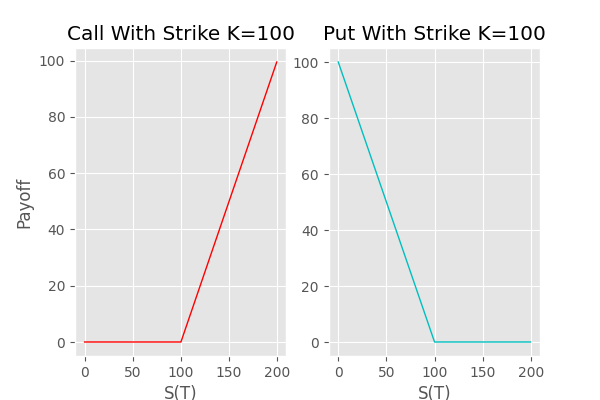
\includegraphics{Figures/contractfct.png}\\
\decoRule
\caption[Contract Functions]{European options payoff at maturity with strike K=100}
\label{fig:contractfct}
\end{figure}

From the above illustration is it clear, that the owner of the option has limited downside, but the illustation does not take into account the initial price for the option. The profit and loss ($P\& L$) graph is also a common way of illustrating the payoff for an option, where you take the initial cost of buying the option into account. The fair price for such type of contract and other contracts will be the topic for this thesis, where the concepts of completeness and arbitrage will be central.

%-----------------------------------
%	SUBSECTION 2
%-----------------------------------

\subsection{Self-financing Portfolio (Without Consumption)}
Before being able to use the concepts of arbitrage and compleness, the construction of the portfolio from the financial market model will be important. The portfolio is the number of each assets of the market the owner of the portfolio holds. The value of the portfolio for a market model with the bank account and d stocks:
\begin{equation}
V^h(t)=\sum_{i=0}^{d} h_{i}(t) S_i(t)
\end{equation}
$V^h$ is called the value process and $h_i(t)$ is number of shares of type i during the period "$[t,t+dt)$". For the definition of arbitrage (Definition \ref{Arbitrage}) we need to restrict ourselfes to self-financing (S-F) portfolios. A self-financing portfolio h, is a portfolio h which doesn't get any external injection of money.
\theoremstyle{definition}
\begin{definition}{Self-financing portfolio}
A portfolio consisting of d+1 assets: \\
h(t)=($h_0(t),h_1(t), \dotsc, h_{d}$) is self-financing if:
\begin{equation}\label{SF}
\begin{split}
dV^{h}(t)=\sum_{i=0}^{d} h_{i}(t) dS_{i}(t)
\end{split}
\end{equation}
Where $S_{i}$ is the $i'th$ asset in our portfolio, d+1 is the total number of assets in our market model and\\
$V^{h}(t)=\sum_{i=0}^{n} h_{i}(t) S_{i}(t)$
\end{definition}
When dealing with discrete time finance the S-F portfolio is actually a budget restriction, this is important intuition for the continuous time version, because the continuous time version can be thought of the limit of the discrete version by letting step sizes in time tending to zero. To avoid pathological effects on the portfolio one often introduce the concept of an admissible portofolio:
\theoremstyle{definition}
\begin{definition}{a-admissible portfolio}
For $a\geq 0$, a portfolio h is called a-admissible if its value process $V^h(t)$ is uniform bounded from below by -a. A portfolio h is admissible if it is a-admissible for some $a\geq 0$.
\end{definition}
The definition of a-admissible portofolio avoid situations as the doubling strategy known from gambling and imposes a limit to the debt arrangement. The important takeaway is that the S-F portfolio you only reallocate your assets through time within the portfolio.

%-----------------------------------
%	SUBSECTION 3
%-----------------------------------
\subsection{Arbitrage}
Arbitrage is the financial term for a "free lunch". An arbitage opportunity produces something out of nothing without risk, where the efficient market assumptions tells us in a well function market the "money pumps" cannot exist for long, because they would quickly be corrected by exploitation. In order to avoid making a "money machine" in our market, we want to price derivatives by not introducing arbitrage to the market.  
\theoremstyle{definition}
\begin{definition}{\textbf{Arbitrage}:}
An arbitrage possibility on a financial market is an admissible self-financed portfolio h suct that
\begin{equation}\label{Arbitrage}
\begin{split}
V^{h}(0)=0\\
P(V^{h}(T)\geq 0)=1\\
P(V^{h}(T)>0)>1
\end{split}
\end{equation}
The financial market $\bm{S}$ is called arbitrage-free if there exist no arbitrage opportunities. Sometimes $\bm{S}$ is said to satisfy (\textit{NA})\\
(p. 96 \parencite{finKont})
\end{definition}
From the above definition we see that arbitrage is a natural financial requirement for a financial market model, because the investor in a arbitrage portfolio starts with 0 dollars, and without injecting any money, the investor is certain of not losing any money. In addition he has a positive probability by ending up with more than 0 at maturity. To price the derivatives fair in the model, the derivative should not introduce arbitrage to the market. There are different versions of the (\textit{NA}) definition, where for our purpose the above defition is sufficient. The \textit{NA} is not only desirable for the market, we would also like to be able to replicate the payoff of the derivative with the other assets in the financial market model. If every derivative can be replicated in the market, then we have a complete market.

%-----------------------------------
%	SUBSECTION 4
%-----------------------------------

\subsection{Complete Market And Hedging}
Hedging is an important topic for risk management, because it tells you have to risk neutralize your exposure, i.e. a hedge is simply a risk neutralization action in order to minimize the overall risk. In the definition below, we define a hedge for an simply T-claim.
\theoremstyle{definition}
\begin{definition}{\textbf{Hedging and completeness for T-claim}:}
A T-claim X can be hedged, if there exist a self-financing portfolio h such that:
\begin{enumerate}
\item[•] $V^{h}(T)=X$ P-a.s.
\end{enumerate}
I.e. h is an hedge portfolio for X if it is guaranteed to pay in all circumstances an amount identical to the payout of X.\\
The market is complete, if every derivative is hedgeable.
(p. 192 \parencite{finKont})
\end{definition}
By introducing the basic concepts for how to price fair and protect ourselves against financial risk, we will in next section focus on building the financial market model.

%----------------------------------------------------------------------------------------
%	SECTION 2
%----------------------------------------------------------------------------------------

\section{Multidimensional Models}\label{MultiDimModel}
There is two main method for deriving arbitrage free and complete markets. The classical approach is the delta hedging approach \parencite{B-S-Paper} and \parencite{CRR}). The more advanced mathematical approach is the martingale approach  \parencite{finKont}. In this section we will focus on the martingale approach and show that delta hedging approach is a special case of the more general martingale theory. For the martingale approach the First and Second Fundamental Theorems of Mathematical Finance will be the key for obtaining a fair market. Besides the model assumptions will we also assumes the financial market assumptions in section \ref{FinMarket}.

\subsection{Model Assumptions}
Let us consider a filtered probability space $(\Omega, \mathcal{F}, P, \mathcal{F}_t^{\bar{W}})$. Note the assumption that filtration is generated from the Wiener process, so the $\bar{W}$ is the only random source and we assume $\bar{W}_i$ is k-dimensional. I.e. we assume that we are in a Wiener world, where all processes are Wiener driven. A priori we assume a market $(B(t),S_1(t), S_2(t),\ldots, S_d(t))$, where ${S_i(t)}_{i=1,2,\ldots,d}$ are d risky assets and B(t) is the risk free asset. By assumptions their dynamics are given by:\\
\begin{align}
d\bm{S}(t)=D[\bm{S}(t)]\bm{\alpha}(t)dt+D[S(t)]\bm{\sigma}(t)d\bar{\bm{W}}(t)\label{GBM-P} \\
dB(t)=r(t)B(t)dt
\end{align}
We assume $\alpha_i$, $\sigma_{ij}$ and the short rate $r(t)$ are adapted processes. The evolution of the stocks are described by a geometric brownian motion (GBM) which has a solution to the SDE. The randomness comes from the brownian motion (BM) in the GBM, which has wildly tracjectories. The function $t\mapsto W_{t}(\omega)$ from $[0,\infty)$ to $\mathbb{R}$ is continuosus, but nowhere differentiable. Furthermore has the BM nonzero quadratic variation and infinite variation, but it also process well-behaved property e.g. the BM is a Lévy process. For illustation figure \ref{fig:BM} we plottet three approximations to three sample paths of the GBM with initial value $S_{i}(0)=36$.

\begin{figure}[H]
\centering
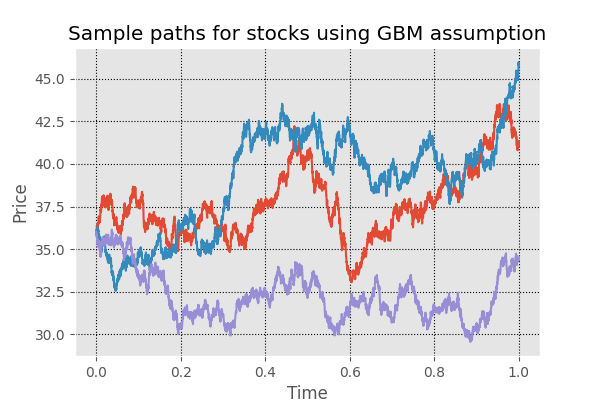
\includegraphics{Figures/samplePath.png}
\decoRule
\caption[Sample Path For Stocks]{Three sample paths for stocks under GBM assumptions, where the spot is \$36, $\sigma$=0.2 and $\alpha$=0.06}
\label{fig:BM}
\end{figure}

The tool for handling BM is stochastic calculus in continuous time, because the standard calculus will not work for the wildly behaved BM. In the representation of the GBM, we used vector and matrix notation for the GBM process. The stock vector is d dimensional and the wiener process vector is k dimensional. The volatility matrix is given by $\bm{\sigma}=\{\sigma_{ij}(t)\}_{i=1,\ldots,d,j=1,\ldots,k}$ and the local mean of rate of return vector is $\alpha=(\alpha_1(t), \alpha_2(t), \ldots, \alpha_d(t))^T$. D(x) denotes a diagonal matrix with vector x as its diagonal and the Wiener processes covariance is $Cov(dW_i(t)dW_j(t))=\rho_{ij}dt$ where $\rho_{i,i}=1$

\subsection{Arbitrage Free Model}
The first problem we are faced with in arbitrage theory is to create a model with no arbitrage opportunities. The First Fundamental Theorem tells us how to not introduce arbitrage to our market model.
\begin{theorem}\label{FFT1}
\textbf{First Fundamental Pricing Theorem of Mathematical Finance(FFT1): } The market model is free of arbitrage if and only if there exist a equivalent martingale measure, i.e. a measure $Q\sim P$ s.t. the processes:
$$\frac{S_0(t)}{S_0(t)}, \frac{S_1(t)}{S_0(t)}, \cdots, \frac{S_d(t)}{S_0(t)}$$
are (local)martingales under Q.
(see p. 154 \parencite{finKont})
\end{theorem}

From the FFT1 with the bank account B(t) as numeraire, we have:
\theoremstyle{proposition}
\begin{proposition}{}
We assume that $B(t)=S_0(t)$ is our numeraire and all the processes are Weiner driven, then a equivalent measure $Q \sim P$ is martingale measure if and only if all assets $(B(t), S_1(t), \ldots, S_d(t))$ have the short rate as their local rates of return, i.e.
\begin{align}
dS_i(t)=S_i(t)r(t)dt+S_i(t)\sigma_i(t)dW^Q(t)
\end{align}
(see p. 154 \parencite{finKont})
\end{proposition}
So to not introduce arbitrage to the model for the financial market, we need to ensure the Q-dynamics of S is:
\begin{equation}\label{Q-dym}
dS(t)=D[S(t)]r(t)dt+D[S(t)]\sigma(t)d\bar{W}(t)
\end{equation}
The tool to obtain the dynamics in eq. (\ref{Q-dym}) is Girsanov theorem (see \ref{Girsanov}). Girsanov theorem is a continuous measure transformation, where in our model we want to transform the dynamics given with the objective probability measure P to an equivalent martingale measure Q (i.e. the martingale measure chosen by the market). By suitable chooses of the likelihood process L and setting $dQ=L(T)dP$, then with Girsanov theorem:
$$d\bar{W}(t)=\phi(t)dt + dW(t)$$
When applying to eq. (\ref{GBM-P}):
$$dS(t)=D[S(t)](\alpha(t)+\sigma(t)\phi(t))dt+D[S(t)]\sigma(t)d\bar{W}(t)$$
Going back to the FFT1 and the proposition, we know that Q is martingale measure if and only if:
\begin{align}\label{marketPriceOfRisk}
\bm{\alpha}(t)+\bm{\sigma}(t)\bm{\phi}(t)=\textbf{r}(t) \quad holds \ with \ probability \ 1 \ for \ each \ t
\end{align}
We disregard pathological models when doing so the term generically arbitrage free will be used. 

\theoremstyle{definition}
\begin{definition}{\textbf{Generically arbitrage free}:}
The model in this section is said to be generically arbitrage free if it is arbitrage free for every (sufficiently integrable) choice of $\bm{\alpha}$.
(p. 198 \parencite{finKont})
\end{definition}

Furthermore we assume enough integrability and we have the following useful result:
\theoremstyle{proposition}
\begin{proposition}{}\label{arbitrageFreeProp}
Disregarding integrability problems the model is generically arbitrage free if and only if, for each $t\leq T$ and P-a.s. the mapping:
$\bm{\sigma}(t):\mathbb{R}^k \to \mathbb{R}^n$ is surjective, i.e. if and only if the volatility matrix $\bm{\sigma}(t)$ has rank n.
(see p. 198 \parencite{finKont})
\end{proposition}
We note that in order not to have arbitrage in our model, we need $k\geq n$, i.e. have at least as many random sources as number of risky assets.

\subsection{Complete model}
Second Fundamental Pricing Theorem is key to obtain a complete market model, i.e. a market model where every claim can be hedged.
\begin{theorem}\label{FFT2}
\textbf{Second Fundamental Pricing Theorem of Mathematical Finance(FFT2): } Assuming absence of arbitrage, the market model is complete if and only if the martingale measure $Q$ is unique.
(see p. 155 \parencite{finKont})
\end{theorem}
Hence in our Wiener world we have a unique martingale measure if eq. \ref{marketPriceOfRisk} has a unique solution. 

\begin{proposition}{}\label{completeProp}
Assume that the model is generically arbitrage free and that the filtration is defined by:
$$\mathcal{F}_t=\mathcal{F}_t^{\bar{W}}$$
Then disregarding integrability problems, the model is complete if and only if k=n and the volatility matrix $\sigma(t)$ is invertible P-a.s. for each $t \leq T$
(see p. 200 \parencite{finKont})
\end{proposition}


\subsection{Pricing and connection to classical approach}
The pricing formula for arbitrage free market model is the risk neutral valuation formula:
\begin{proposition}{}\label{RNVF}
To avoid arbitrage, $\mathcal{X}$ must be priced according to the formula:
\begin{align}
\Pi(t;\mathcal{X})=S_0(t)E^Q[\frac{\mathcal{X}}{S_0}|\mathcal{F}_t]
\end{align}
Note if we choose our numeraire $S_0(t)=B(t)$ then
\begin{align}
\Pi(t;\mathcal{X})=E^Q[\exp(-\int_t^T r(s) ds) \mathcal{X}|\mathcal{F}_t]
\end{align}
(see p. 155 \parencite{finKont})
\end{proposition}

The classical approach to arbitrage free and complete market models is based on a Markovian model assumption and k=n. Assume we are in a Wiener world, where the probability space $(\Omega, \mathcal{F}, P, \mathcal{F}_t^{\bar{W}_t}$ is given. Furthermore we assume $\alpha$ and $\sigma$ are deterministic functions and constant over time. $\sigma$ is also assumed invertible. Under these more restrictive assumptions the risk neutral valuation formula for a simple T-claim is given by the Markov property:
\begin{align}\label{MarkovRNVF}
\exp(-r(T-t))E^Q[\mathcal{X}|S(t)]
\end{align}

Applying Kolmogorov backward equation on eg. \ref{MarkovRNVF}, we obtain the BS-PDE for the pricing function F(t,S(t))=$\Pi(t; \mathcal{X})$.

\begin{theorem}\label{BSPDEMultiDim}
\textbf{Black Scholes PDE: } Consider the contract $\mathcal{X}=\Phi(\bm{S}(T))$. In order not to introduce arbitrage to the market, the pricing function $F(t,s)$ must solve the boundary value problem.
\begin{equation}
\begin{split}
F_t(t,s)+\sum_{i=1}^{n} rs_iF_i(t,s)+\frac{1}{2} tr\{\sigma^* D[S] F_{ss} D[S] \sigma\} -rF(t,s)&=0\\
F(T,s)&=\Phi(s)
\end{split}
\end{equation}
(see p. 203 \parencite{finKont})
\end{theorem}


%----------------------------------------------------------------------------------------
%	SECTION 3
%----------------------------------------------------------------------------------------
\section{Classical Black-Scholes Formulas}\label{classicBS}
We will not do the classical delta hedging approach in \parencite{B-S-Paper}. Instead we use the general multidimensional martingale approach to derive the essential formulas for pricing. 
To derive a closed-form solution to the European call and put option, we concentrate at a special case of the multidimensional framework, where we only have the risk free asset and one risky asset. 
We further restrict ourselves to:\\
\theoremstyle{assumption}
\begin{assumption}{Black-Scholes assumptions}\label{BS-Assumption}
We assume following ideal conditions in addition to \eqref{EfficientMarket}:
\begin{enumerate}
\item[•] The short-term interest rate is known and is constant through time 
\item[•] The stock price follows a Geometric Brownian Motion. The $\sigma$ is constant.\item[•] The stock pays no dividends or other distributions.
\item[•] The option is a simple option ("European" see \eqref{ECall}).
\end{enumerate}
(see p. 640 \parencite{B-S-Paper})
\end{assumption}

We assume the underlying stock follows a geometric brownian motion:
$dS(t)=\alpha S dt + \sigma S dW_t$ where the solution to the SDE is given as
\begin{equation}\label{GBM}
\begin{split}
S(t)=S(0) \cdot \exp \bigg( (\alpha -\frac{1}{2} \sigma^2) t + \sigma W(t) \bigg)
\end{split}
\end{equation}
Where $\alpha$ is the local mean rate of return and $\sigma$ is the volatility of S. By above assumptions we are in a Markovian model, and we know the Black Scholes PDE in this setup (see eq.  \ref{BSPDEMultiDim}). By Feynman-Kac we have the risk neutral valuation formula.

\begin{theorem}\label{BRNVF}
\textbf{Risk-neutral valuation formula:} Given Q is the martingale measure
\begin{align}
\Pi(t, X)= exp(-r(T-t))\cdot E_{t,x}^Q[X]
\end{align}
\end{theorem}
From the RNVF we can derive a closed form solution for both a European call and put option. We will provide the European call option and the put-call-parity, because from the put-call-parity relationship we derive the European put option from the call option.

\theoremstyle{proposition}
\begin{proposition}{}\label{BS-price-EuroCall}
\textbf{Black-Scholes formula for call option:} The price of a European call option with strike K and maturity T is given by the formula  $\Pi(t)=F(t,S(t)$, where
\begin{align*}
F(t,s)=s \cdot N(d_1(t,s)) - e^{-r(T-t)}\cdot K \cdot N(d_2(t,s))
\end{align*}
N is the cumulative distribution function of a standard normal distribution $\mathcal{N}(0,1)$ and
\begin{align*}
d_1(t,s)=\frac{1}{\sigma\cdot \sqrt{T-t}} \cdot \bigg( \ln(\frac{s}{K}) + (r+\frac{1}{2} \sigma^2) (T-t) \bigg)\\
d_2(t,s)=d_1(s,t)-\sigma \sqrt{T-t}
\end{align*}
(see p. 105 \parencite{finKont})
\end{proposition}

\theoremstyle{proposition}
\begin{proposition}{}\label{put-call-parity}
\textbf{Put-call parity:} 
Assume the call and put option has same strike price and time to maturity.
\begin{align*}
p(t,s)=K\cdot \exp(-r(T-t))+c(t,s)-s
\end{align*}
(see p. 126 \parencite{finKont})
\end{proposition}

The put-call-parity holds only for European options, but the framework developed in this section will be useful for benchmarks and control variate for the numerical procedures.

The above formula for the European call option is actually the same for an American call option, but is not true for an American put option or for call options paying dividends. The result for the American call option was shown by Merton \parencite{Merton73}, that the intrinsic value is never greater than the worth of the option given by the risk-neutral valuation formula. In section \ref{AmericanOptions} we will show a martingale approach to prove the value of a European and American call coincides when the underlying is a non-dividend paying stock \parencite{finKont}.

%----------------------------------------------------------------------------------------
%	SECTION 4
%----------------------------------------------------------------------------------------

\section{American Options And Optimal Stopping}\label{AmericanOptions}
The American options adds additional complexity to the pricing problem, because compared to the European option the American option can be exercised at any time from inception to maturity. The main problem with American options is to find a optimal stopping time, i.e.
\begin{align}
\max_{0 \leq \tau\leq T}\{E[\Phi(\tau,X_{\tau})]\}
\end{align}
Where $\tau$ is a stopping time (see definition \ref{stopTime}).
We assume satisfied integrability condition on a finite interval $[0,T]$:
$$\sup_{0 \leq \tau\leq T}\{E[\Phi(\tau,X_\tau)]\}<\infty$$
and assume a diffusion setting:
$$dX_t=\mu(t,X(t))dt + \sigma(t,X(t))dW(t)$$

To find the optimal stopping time we introduce the optimal value function V(t,X(t)).
\theoremstyle{definition}
\begin{definition}{Optimal value function }\label{optValFunc}
For fixed $(t,x)\in [0,T]X\mathbb{R}$, and each stopping time $\tau$ with $\tau\geq t$ the optimal value function $V(t,x)$ is defined by
\begin{align}
V(t,x)=\sup_{t \leq \tau\leq T}\{E[\Phi(\tau,X_{\tau})]\}
\end{align}
A stopping time which realizes supremum for V is called optimal and be denoted $\hat{\tau}_{tx}$.
(see page 341 \parencite{finKont})
\end{definition}
By using a dynamic programming argument with three strategies:
\begin{enumerate}
\item[•] Use optimal stopping strategy $\hat{\tau}_t$
\item[•] Stop immediately
\item[•] Wait one time-step h and then use optimal stopping strategy $\hat{\tau}_{t+h}$
\end{enumerate}
Jumping over some argument and like in this section assuming "enough regularity", we arrive at two important propositions for numerically evaluating American options.

\begin{proposition}{\textbf{variational inequalities}}\label{varInEq}
Given enough regularity, the optimal value function is characterized by the following relations:
\begin{equation}
\begin{split}
V(T,x)=\Phi(T,x)\\
V(t,x)\geq \Phi(t,x) \quad \forall (t,x)\\
\bigg(\frac{\partial}{\partial t} + \mathbb{A}\bigg)V(t,x) \leq 0 \quad \forall (t,x)\\
\max\bigg\{V(t,x) - \Phi(t,x), \bigg(\frac{\partial}{\partial t} + \mathbb{A}\bigg)V(t,x) \bigg\} = 0 \quad \forall (t,x)\\
\textsl{Where $\mathbb{A}$ is the Itô operator:}\\
\mathbb{A}f(t,x) =  \mu(t,x) \frac{\partial f(t,x)}{\partial x} + \frac{1}{2} \sigma^2(t,x) \frac{\partial^2 f(t,x)}{\partial x^2}
\end{split}
\end{equation}
(see p. 344 \parencite{finKont})
\end{proposition}

\begin{proposition}{\textbf{Free boundary value problem}}\label{freeBoundary}
Assuming enough regularity, the optimal value function satisfies the following parabolic equation
\[ \begin{cases} 
      \frac{\partial V(t,x)}{\partial t}(t,x) + \mu(t,x) \frac{\partial V(t,x)}{\partial x}(t,x) + \frac{1}{2}\sigma^2(t,x)\frac{\partial^2 V(t,x)}{\partial x^2}=0 & (t,x)\in C \\
     V(t,x)=\Phi(t,x)  & (t,x)\in \partial C \\
   \end{cases}
\]
Where C is the continuation region defined by:
$$C=\{(t,x): V(t,x)>\Phi(t,x) \}$$
(see p. 343-344 \parencite{finKont})
\end{proposition}

We will see in the American put section why these two propositions are useful.

\subsection{American Call Without Dividends}
The American call options is a special case, because the optimal stopping time is always at the options maturity. With martingale machinery it means the value-process is a submartingale, which mean the $\hat{\tau}=T$.

The optimal stopping problem is:
$$\sup_{0 \leq \tau\leq T}\{E[\exp(-r \tau) \max\{S_{\tau} - K, 0\}]\}$$
Hence we want to maximize the expectation of the process:
$$ \max\{ \exp(-r t) S_{t} - \exp(-r t) K, 0 \}$$

From the theory developed we know that $\exp(r\cdot t) \cdot S_t$ is a Q-martingale and $\exp(r\cdot t) \cdot K$ is a deterministic decreasing function hence a supermartingale. Then $\exp(r\cdot t) \cdot S_t - \exp(r\cdot t) \cdot K$ is a submartingale. Applying the function max which is a convex and increasing functionther on a submartingale is still a submartingale. Hence the optimal stopping time is $\hat{\tau}=T$.

\subsection{American Put}
For the American put the optimal stopping problem is:
$$\max_{0 \leq \tau\leq T}\{E[\exp(-r \tau) \max\{K - S_{\tau}, 0\}]\}$$
There is no analytical formula for American put, hence numerical procedures are required. For practical use there are three strategies to find the fair price for the option:
\begin{enumerate}
\item[•] Solve the free boundary free problem numerically (see \ref{freeBoundary})
\item[•] Solve the variational inequalities numerically (see \ref{varInEq})
\item[•] Approximate the Black-Scholes model by a binomial model and compute the exact binomial American put price.
\end{enumerate}
\parencite{finKont}\\

We will in the following chapters try to valuate with both the binomial model and solving the variational inequalities.